%-----------------------------------------------------------------------------
%   Copyright 2013 Florian Schumacher
%
%   This file is part of the ASKI manual as a LaTeX document with main file
%   manual.tex
%
%   Permission is granted to copy, distribute and/or modify this document
%   under the terms of the GNU Free Documentation License, Version 1.3
%   or any later version published by the Free Software Foundation;
%   with no Invariant Sections, no Front-Cover Texts, and no Back-Cover Texts.
%   A copy of the license is included in the section entitled ``GNU
%   Free Documentation License''. 
%-----------------------------------------------------------------------------
%
In general, in this chapter we provide only basic information. For more detail on 
specific steps or objects, we always refer to the respective sections below in this document.
%
%++++++++++++++++++++++++++++++++++++++++++++++++++++++++++
\section{Installing \ASKI} \label{basic_steps,sec:install_ASKI}
%++++++++++++++++++++++++++++++++++++++++++++++++++++++++++
%
\begin{itemize}
\item Download here: \url{http://www.rub.de/ASKI}
\item Unpack tar ball somewhere
\item Follow the directions in file \lcode{ASKI_0.3/README}
\end{itemize}
%
%++++++++++++++++++++++++++++++++++++++++++++++++++++++++++
\section{Create Main Parameter File} \label{basic_steps,sec:main_parfile}
%++++++++++++++++++++++++++++++++++++++++++++++++++++++++++
%
The simplest way to create a specific main parameter file for your operation is to modify / adjust 
a copy of the template file \lcode{template/main_parfile_template}. 

Refer to the commented documentation in \lcode{main_parfile_template} or 
to sections~\myref{files,sec:parfiles} and~\myref{files,sec:main_parfile}.
%
%++++++++++++++++++++++++++++++++++++++++++++++++++++++++++
\section{Iteration Step Parameter Files} \label{basic_steps,sec:iter_parfile}
%++++++++++++++++++++++++++++++++++++++++++++++++++++++++++
%
Having created a directory environment for your operation, as described in section~\myref{basic_steps,sec:create_dir},
there should automatically have been created template
parameter files in each directory of an iteration step, having filenames as defined by
parameter \lcode{PARFILE_ITERATION_STEP} in the main parameter file.

Refer to the commented documentation in those template files or 
to sections~\myref{files,sec:parfiles} and~\myref{files,sec:iter_parfile}.
%
%++++++++++++++++++++++++++++++++++++++++++++++++++++++++++
\section{Create Directory Environment} \label{basic_steps,sec:create_dir}
%++++++++++++++++++++++++++++++++++++++++++++++++++++++++++
%
Call python script \lcode{create_ASKI_dir.py}
\begin{lstlisting}
USAGE: please give 2 arguments:
[1] main parmeter file of inversion
[2] number of iteration steps

EXAMPLE:
create_ASKI_dir.py ./main_parfile_Aegean1 10
\end{lstlisting}
Put your main parameter file (see~\myref{basic_steps,sec:main_parfile}) as the first, and the expected 
number of iteration steps as the second argument. \\
You can always \emph{recall this script at any later time} with a larger number of iteration steps. 
All existing directories \emph{will not be affected}, only additional non-existing objects will be 
created. Recalling this script with a smaller number of steps will not delete anything.
%
%++++++++++++++++++++++++++++++++++++++++++++++++++++++++++
\section{Data in \ASKI} \label{basic_steps,sec:data_general}
%++++++++++++++++++++++++++++++++++++++++++++++++++++++++++
%
One certain data sample in \ASKI is characterized by a seismic \emph{source}, a \emph{component} 
of a seismic \emph{receiver}, and a \emph{frequency}, as well as if it is \emph{real} or \emph{imaginary} part 
of the complex spectral values. It has the value of displacement of the ground in the unit of meters.
%
%----------------------------------------------------------
\subsection*{Events and Receivers}
%----------------------------------------------------------
%
The events file (\myref{files,sec:event_list}) and stations file (\myref{files,sec:station_list}) constitute a
collection of \emph{all} events (stations) which will be involved \emph{in any way} in your \ASKI operation.\\
All programs/scripts will refer to a specific event (station) by its event-ID (station-name).
%
%----------------------------------------------------------
\subsection*{Receiver Components}
%----------------------------------------------------------
%
All programs/scripts will refer to a specific receiver component by the following abbreviatory names.\\
Dependent on the coordinate system in which the receivers are defined (Cartesian or spherical, which is 
defined by the first line of the station list file), the supported names of receiver components may have a 
different meaning:
\subsubsection{Cartesian receivers}
\begin{itemize}
\item[] \lcode{CX}: Cartesian \lcode{X}-coordinate (first Cartesian coordinate)
\item[] \lcode{CY}: Cartesian \lcode{Y}-coordinate (second Cartesian coordinate)
\item[] \lcode{CZ}: Cartesian \lcode{Z}-coordinate (third Cartesian coordinate)
\item[] \lcode{N}: same as \lcode{-CX}
\item[] \lcode{S}: same as \lcode{CX}
\item[] \lcode{E}: same as \lcode{CY}
\item[] \lcode{W}: same as \lcode{-CY}
\item[] \lcode{UP}: same as \lcode{CZ}
\item[] \lcode{DOWN}: same as \lcode{-CZ}
\end{itemize}
\subsubsection{Spherical receivers}
\begin{itemize}
\item[] \lcode{CX}: Cartesian \lcode{X}-coordinate with \lcode{X}-axis through equator and $0^\circ$-meridian
\item[] \lcode{CY}: Cartesian \lcode{Y}-coordinate with \lcode{Y}-axis through equator and $90^\circ$E-meridian
\item[] \lcode{CZ}: Cartesian \lcode{Z}-coordinate with \lcode{Z}-axis through north pole
\item[] \lcode{N}: local north
\item[] \lcode{S}: local south
\item[] \lcode{E}: local east
\item[] \lcode{W}: local west
\item[] \lcode{UP}: local up
\item[] \lcode{DOWN}: local down
\end{itemize}
%
%----------------------------------------------------------
\subsection*{Frequency Discretization}
%----------------------------------------------------------
%
In \ASKI, frequencies are given by a frequency step $\Delta f$[Hz] and by a set of integer valued 
frequency indices.

For specific frequency index $i$, the corresponding frequency $f_i$ [Hz] computes as $f_i \,=\, i \,\cdot\, \Delta f$.
E.g.\ $\Delta f \,=\, 10$ Hz and frequency indices $i \,=\, 2,\; 3,\; 5,\; 7,\; 10$ define the set of 
discrete frequencies $f_i \,=\, 20.0,\; 30.0,\; 50.0,\; 70.0,\; 100.0$ [Hz].
%
%++++++++++++++++++++++++++++++++++++++++++++++++++++++++++
\section{Prepare Measured Data} \label{basic_steps,sec:measured_data}
%++++++++++++++++++++++++++++++++++++++++++++++++++++++++++
%
{\bf In the future}, we plan to have a binary program \lcode{createMeasuredData}, which converts time-domain data 
to the special frequency-domain form required by \ASKI. It is planned to supporte measured data given in some 
basic data formats like Seismic Unix and time-series given as textfiles per trace.

For now, you must prepare measured data files on your own as required by \ASKI, see sections~\myref{basic_steps,sec:data_general} 
and~\myref{files,sec:measured_data}. 
%
%++++++++++++++++++++++++++++++++++++++++++++++++++++++++++
\section{Define an Inversion Grid} \label{basic_steps,sec:invgrid}
%++++++++++++++++++++++++++++++++++++++++++++++++++++++++++
%
There are different types of \ASKI inversion grids suitable for different geometries, 
forward methods, hence, applications.

All inversion grids are defined by setting parameters \lcode{TYPE_INVERSION_GRID} and 
\lcode{PARFILE_INVERSION_GRID} in the parameter file of the current iteration step.

In the following, we present the supported inversion grid types and explain the particular
parameters in the respective inversion grid parameter file.
%
%----------------------------------------------------------
\subsection{\lcodetitle{scartInversionGrid}} \label{basic_steps,sec:invgrid,sub:scart}
%----------------------------------------------------------
%
A \lcode{S}imple \lcode{CART}esian inversion grid covers a Cartesian cuboid which can
be shifted to a certain location in Cartesian space and may be rotated about the local vertical
axis. Its cells are distributed in layers. Each layer has a certain thickness and a regularly
distributed number of inversion grid cells along each lateral direction of the cuboid.

Please consult the documentation of your forward method (\myref{basic_steps,sec:forward_problem}) if it supports
inversion grids of type \lcode{scartInversionGrid}. \\
All coordinates, e.g.\ of events and stations or wavefield points, are interpreted by this type of inversion grid as
\lcode{X} (first coordinate), \lcode{Y} (second coordinate), \lcode{Z} (third coordinate). Their
units (e.g.\ meters or kilometers) are not assumed by the inversion grid and are essentially defined by the wavefield
points, hence, they might be method dependent and must be overall consistend.\\
Every type of integration weights is supported by this type of inversion grid, except weights of type 
\lcode{6} (external integration weights).

\begin{figure}[ht]
  \centering
  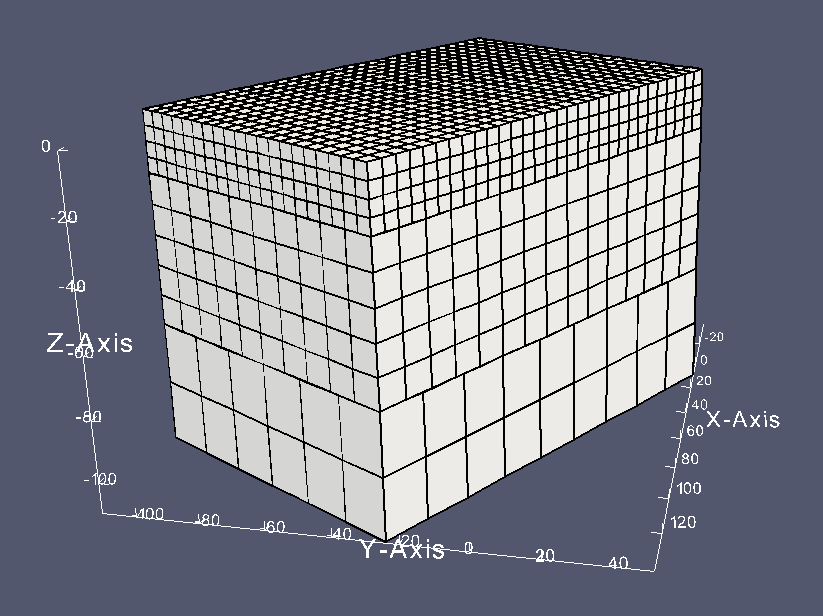
\includegraphics[width=0.5\textwidth]{images/scartInversionGrid_manual.png}
  \caption{Example of a simple Cartesian inversion grid}
  \label{basic_steps,sec:invgrid,sub:scart,fig:grid}
\end{figure}

The shape of the cuboid, as well as the distribution of inversion grid cells, are defined 
via a paramter file, a template of which is file \lcode{template/scartInversionGrid_parfile_template}.
In the following, the particular parameters are explained, with the example
values always refering to the inversion grid as displayed in figure~\myref{basic_steps,sec:invgrid,sub:scart,fig:grid}.

%- - - - - - - - - - - - - - - - - - - - - - - - - - - - - 
\subsubsection{\lcode{SCART_INVGRID_CX}}
\lcode{X}-coordinate of center of cuboid (real number)\\
Example:\\
\lcode{SCART_INVGRID_CX = 50.0}
%- - - - - - - - - - - - - - - - - - - - - - - - - - - - - 
\subsubsection{\lcode{SCART_INVGRID_CY}}
\lcode{Y}-coordinate of center of cuboid (real number)\\
Example:\\
\lcode{SCART_INVGRID_CY = -30.0}
%- - - - - - - - - - - - - - - - - - - - - - - - - - - - - 
\subsubsection{\lcode{SCART_INVGRID_ZMAX}}
Maximum \lcode{Z}-coordinate of cuboid (real number), i.e.\ \lcode{Z}-coordinate of the 
``surface'' of the inversion grid\\
Example:\\
\lcode{SCART_INVGRID_ZMAX = 0.0}
%- - - - - - - - - - - - - - - - - - - - - - - - - - - - - 
\subsubsection{\lcode{SCART_INVGRID_WX}}
Width of cuboid in \lcode{X}-direction (real number)\\
Example:\\
\lcode{SCART_INVGRID_WX = 100.0}
%- - - - - - - - - - - - - - - - - - - - - - - - - - - - - 
\subsubsection{\lcode{SCART_INVGRID_WY}}
Width of cuboid in \lcode{Y}-direction (real number)\\
Example:\\
\lcode{SCART_INVGRID_WY = 150.0}
%- - - - - - - - - - - - - - - - - - - - - - - - - - - - - 
\subsubsection{\lcode{SCART_INVGRID_ROT}}
Angle in degrees of anti-clockwise rotation about the local \lcode{Z}-axis through the 
lateral center of the cuboid (real number)\\
Example:\\
\lcode{SCART_INVGRID_ROT = 60.0}
%- - - - - - - - - - - - - - - - - - - - - - - - - - - - - 
\subsubsection{\lcode{SCART_INVGRID_NREF_BLOCKS,SCART_INVGRID_NLAY,SCART_INVGRID_THICKNESS}}
For an arbitrary number of \lcode{SCART_INVGRID_NREF_BLOCKS} blocks of layers,
the vectors \lcode{SCART_INVGRID_NLAY} (integer values) and \lcode{SCART_INVGRID_THICKNESS} (real values), 
both of length \lcode{SCART_INVGRID_NREF_BLOCKS}, define the \lcode{Z}-direction refinement of each block,
whereby \lcode{SCART_INVGRID_NLAY(i)} defines the number of layers in block \lcode{i}, and 
\lcode{SCART_INVGRID_THICKNESS(i)} defines the thickness of all layers contained in block \lcode{i}.\\
Hence, the overall \lcode{Z}-direction coverage of the inversion grid is defined by 
\lcode{SCART_INVGRID_ZMAX} (which is the coordinate of the top of the first layer in the first refinement block)
and \lcode{SCART_INVGRID_ZMAX - SUM_i(THICKNESS(i) * NLAY(i))} (coordinate of the bottom of the last layer in
%and \lstinline[breaklines=true]$SCART_INVGRID_ZMAX - SUM_i(THICKNESS(i) * NLAY(i))$ (coordinate of the bottom of the last layer in
%and \nolinkurl{SCART_INVGRID_ZMAX - SUM_i(THICKNESS(i) * NLAY(i))} (coordinate of the bottom of the last layer in
last refinement block).\\
Example:\\
\lcode{SCART_INVGRID_NREF_BLOCKS =  3}\\
\lcode{SCART_INVGRID_NLAY =  4   5   2}\\
\lcode{SCART_INVGRID_THICKNESS =  5.0  10.0  20.0}
%- - - - - - - - - - - - - - - - - - - - - - - - - - - - - 
\subsubsection{\lcode{SCART_INVGRID_NX}}
Vector (of length \lcode{SCART_INVGRID_NREF_BLOCKS}) of integer values, defining number of 
inversion grid cells in \lcode{X}-direction, one value for each refinement block\\
Example:\\
\lcode{SCART_INVGRID_NX = 20 10 6}
%- - - - - - - - - - - - - - - - - - - - - - - - - - - - - 
\subsubsection{\lcode{SCART_INVGRID_NY}}
Vector (of length \lcode{SCART_INVGRID_NREF_BLOCKS}) of integer values, defining number of 
inversion grid cells in \lcode{Y}-direction, one value for each refinement block\\
Example:\\
\lcode{SCART_INVGRID_NX = 30 15 9}
%- - - - - - - - - - - - - - - - - - - - - - - - - - - - - 
\subsubsection{\lcode{USE_LOCAL_INVGRID_COORDS_FOR_VTK}}
Logical value to indicate whether to use local inversion grid coordinates for vtk geometry, i.e.\ no rotation 
by \lcode{SCART_INVGRID_ROT} and no shift by \lcode{SCART_INVGRID_CX}, \lcode{SCART_INVGRID_CY}, 
\lcode{SCART_INVGRID_ZMAX} (cuboid centered in \lcode{X=Y=0} and \lcode{ZMAX=0})\\
Example:\\
\lcode{USE_LOCAL_INVGRID_COORDS_FOR_VTK = .false.}
%- - - - - - - - - - - - - - - - - - - - - - - - - - - - - 
\subsubsection{\lcode{SCALE_VTK_COORDS,VTK_COORDS_SCALING_FACTOR}}
Scale vtk geometry coordinates by factor \lcode{VTK_COORDS_SCALING_FACTOR} (real number), if 
\lcode{SCALE_VTK_COORDS = .true.}. This may be helpful if coordinate values (e.g.\ in meters) 
get so large that they cause problems when plotting in paraview.\\
Example:\\
\lcode{SCALE_VTK_COORDS = .false.}\\
\lcode{VTK_COORDS_SCALING_FACTOR = 1.0}
%- - - - - - - - - - - - - - - - - - - - - - - - - - - - - 
%
%----------------------------------------------------------
\subsection{\lcodetitle{ecartInversionGrid}} \label{basic_steps,sec:invgrid,sub:ecart}
%----------------------------------------------------------
%
{\bf WARNING, EXPERIMENTAL FEATURE:} \emph{so far, this type of inversion grid works for tetrahedral cells only,
since support for hexahedreal cells is not completed throughout. However, even for tetrahedra the automatic detection 
of neighbours did not work properly in some test cases! So if you intend to use this inversion grid, please have a look 
at the grid and all neighbours (neighbours only required for model smoothing in case of solving the Kernel system of equations).
You can do that by using binary program} \lcode{invgrid2vtk} \emph{along with option} \lcode{-nb} \emph{. Call} 
\lcode{invgrid2vtk -h} \emph{for further details on how to use it.}

An \lcode{E}xternal \lcode{CART}esian inversion grid is defined by several text files containing the definintion 
of nodes (i.e.\  essentially the corner points, or rather the control nodes of the inversion grid cells) and the 
definition of cells by refering to the nodes. At the moment, 4-node tetrahedral cells are fully supported, and 8-node 
hexahedral cells are partly supported. 
Those files may be produced by any meshing tool. In case you are interested to export meshes your own way, 
section~\myref{files,sec:ecart_invgrid} defines the required file formats.\\
\ASKI provides the \lcode{python} module \lcode{cubit2ASKIecartInversionGrid.py} which can be used with the 
meshing software \lcode{Cubit} in a \lcode{python} script by first importing the module:\\
\lcode{import cubit2ASKIecartInversionGrid}\\
and at the very end of your meshing process calling:\\
\lcode{cubit.cmd('compress all')}\\
\lcode{cubit2ASKIecartInversionGrid.export2ASKI('EXPORT_PATH')}\\
whereby you may replace \lcode{EXPORT_PATH} by some location where the output files will be written.

Please consult the documentation of your forward method (\myref{basic_steps,sec:forward_problem}) if it supports
inversion grids of type \lcode{ecartInversionGrid}. \\
All coordinates, e.g.\ of events and stations or wavefield points, are interpreted by this type of inversion grid as
\lcode{X} (first coordinate), \lcode{Y} (second coordinate), \lcode{Z} (third coordinate). Their
units (e.g.\ meters or kilometers) are not assumed by the inversion grid and are essentially defined by the wavefield
points, hence, they might be method dependent and must be overall consistend.\\
Every type of integration weights is supported by this type of inversion grid, except weights of type 
\lcode{6} (external integration weights).

\begin{figure}[ht]
  \centering
  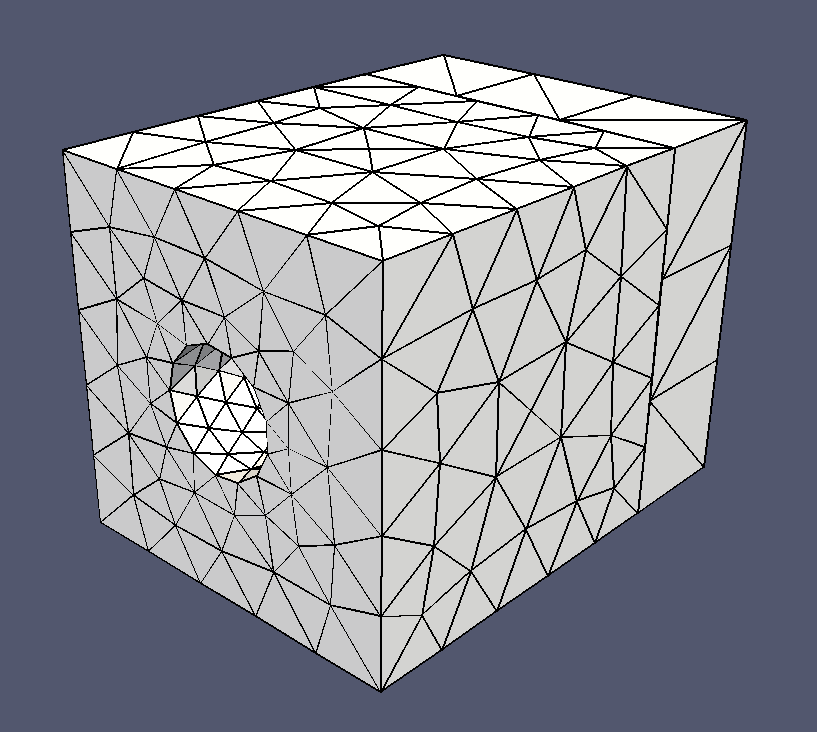
\includegraphics[width=0.5\textwidth]{images/ecartInversionGrid_manual.png}
  \caption{Example of an external Cartesian inversion grid created by Cubit}
  \label{basic_steps,sec:invgrid,sub:ecart,fig:grid}
\end{figure}

The nodes and cell files, e.g.\ produced by \lcode{Cubit}, are referred to in a parameter file, a template 
of which is file \lcode{template/ecartInversionGrid_parfile_template}. In the following, the particular 
parameters are explained. An example inversion grid of this type is displayed in 
figure~\myref{basic_steps,sec:invgrid,sub:ecart,fig:grid}.

%- - - - - - - - - - - - - - - - - - - - - - - - - - - - - 
\subsubsection{\lcode{ECART_INVGRID_USE_NODES_COMMON}}
Logical value to indicate whether to use one common nodes coordinates file for 
all cell types (only use parameter \lcode{ECART_INVGRID_FILE_NODES} below), or to use an individual 
nodes coordinates file for each cell type (use parameters files \lcode{ECART_INVGRID_FILE_NODES_TET4}, 
\lcode{ECART_INVGRID_FILE_NODES_HEX8}, \dots below).\\
When using module \lcode{cubit2ASKIecartInversionGrid} you should set:\\
\lcode{ECART_INVGRID_USE_NODES_COMMON = .True.}
%- - - - - - - - - - - - - - - - - - - - - - - - - - - - - 
\subsubsection{\lcode{ECART_INVGRID_FILE_NODES_COMMON}}
File name relative to \lcode{MAIN_PATH_INVERSION/ITERATION_STEP_PATH/} of nodes coordinates file to be commonly used
for definition of cells of all types in case of \lcode{ECART_INVGRID_USE_NODES_COMMON = .True.}\\
When using module \lcode{cubit2ASKIecartInversionGrid} you should set:\\
\lcode{ECART_INVGRID_FILE_NODES_COMMON = node_coordinates}
%- - - - - - - - - - - - - - - - - - - - - - - - - - - - - 
\subsubsection{\lcode{ECART_INVGRID_FILE_NODES_TET4}}
File name relative to \lcode{MAIN_PATH_INVERSION/ITERATION_STEP_PATH/} of nodes coordinates file to be used
for definition of tet4-type cells in case of \lcode{ECART_INVGRID_USE_NODES_COMMON = .False.}\\
%- - - - - - - - - - - - - - - - - - - - - - - - - - - - - 
\subsubsection{\lcode{ECART_INVGRID_FILE_NODES_HEX8}}
File name relative to \lcode{MAIN_PATH_INVERSION/ITERATION_STEP_PATH/} of nodes coordinates file to be used
for definition of hex8-type cells in case of \lcode{ECART_INVGRID_USE_NODES_COMMON = .False.}\\
%- - - - - - - - - - - - - - - - - - - - - - - - - - - - - 
\subsubsection{\lcode{ECART_INVGRID_FILE_CELLS_TET4}}
File name relative to \lcode{MAIN_PATH_INVERSION/ITERATION_STEP_PATH/} of cell connectivity file for 
definition of tet4-type cells.\\
When using module \lcode{cubit2ASKIecartInversionGrid} you should set:\\
\lcode{ECART_INVGRID_FILE_CELLS_TET4 = cell_connectivity_tet4}
%- - - - - - - - - - - - - - - - - - - - - - - - - - - - - 
\subsubsection{\lcode{ECART_INVGRID_FILE_CELLS_HEX8}}
File name relative to \lcode{MAIN_PATH_INVERSION/ITERATION_STEP_PATH/} of cell connectivity file for 
definition of hex8-type cells.\\
When using module \lcode{cubit2ASKIecartInversionGrid} you should set:\\
\lcode{ECART_INVGRID_FILE_CELLS_HEX8 = cell_connectivity_hex8}
%- - - - - - - - - - - - - - - - - - - - - - - - - - - - - 
\subsubsection{\lcode{ECART_INVGRID_FILE_NEIGHBOURS}}
File name relative to \lcode{MAIN_PATH_INVERSION/ITERATION_STEP_PATH/} of cell neighbours file. If not
present, this file will be created when first using the inversion grid. If present, its content defines 
the neighbour structure of the inversion grid cells. If, however, the inversion grid
is to be recreated (e.g.\ when calling \lcode{initBasics -recr}, see section~\myref{basic_steps,sec:initBasics}),
this file is recreated.
%- - - - - - - - - - - - - - - - - - - - - - - - - - - - - 
\subsubsection{\lcode{ECART_INVGRID_FILE_NEIGHBOURS_IS_BINARY}}
Logical value to indicate whether \lcode{ECART_INVGRID_FILE_NEIGHBOURS} should be binary or not.
%- - - - - - - - - - - - - - - - - - - - - - - - - - - - - 
\subsubsection{\lcode{SCALE_VTK_COORDS,VTK_COORDS_SCALING_FACTOR}}
Scale vtk geometry coordinates by factor \lcode{VTK_COORDS_SCALING_FACTOR} (real number), if 
\lcode{SCALE_VTK_COORDS = .true.}. This may be helpful if coordinate values (e.g.\ in meters) 
get so large that they cause problems when plotting in paraview.\\
Example:\\
\lcode{SCALE_VTK_COORDS = .false.}\\
\lcode{VTK_COORDS_SCALING_FACTOR = 1.0}
%
%----------------------------------------------------------
\subsection{\lcodetitle{specfem3dInversionGrid}} \label{basic_steps,sec:invgrid,sub:specfem3d}
%----------------------------------------------------------
%
An inversion grid of type \lcode{specfem3dInversionGrid} is method dependent and is to be used with 
\lcode{METHOD = SPECFEM3D} only. Whole spectral elements are used as inversion grid cells and all 
GLL points inside such an element as the wavefield points. All information regarding the element 
geometry, including information on neighbour cells and the values of the jacobian for every wavefield 
point contained in an element are read from files which are produced by \lcode{SPECFEM3D} methods.

Every type of integration weights is supported by this type of inversion grid, including weights of type 
\lcode{6} (external integration weights).

Please refer to the documentation of your \lcode{SPECFEM3D} forward method (\myref{basic_steps,sec:forward_problem})
on how to define an inversion grid of type \lcode{specfem3dInversionGrid}.
%
%++++++++++++++++++++++++++++++++++++++++++++++++++++++++++
\section{Define a Starting Model} \label{basic_steps,sec:start_model}
%++++++++++++++++++++++++++++++++++++++++++++++++++++++++++
%
There are two possibilities to define an earth model for the forward wave propagation in your first iteration:

On the one hand you may use any (standard) earth model provided by the forward method you are using, if appropriate.

If this is not possible, or the models provided do not meet your needs, you may use binary 
\lcode{createStartmodelKim} along with the inversion grid of your first iteration (which you should 
have already defined) to produce an inverted model file containing some simple model on this inversion grid. 
\lcode{createStartmodelKim -h} will print a help message how to use the program. Afterwards you may 
export the produced model file to your forward method as explained in section~\myref{basic_steps,sec:export_kim}.
%
%++++++++++++++++++++++++++++++++++++++++++++++++++++++++++
\section{Export Inverted Model} \label{basic_steps,sec:export_kim}
%++++++++++++++++++++++++++++++++++++++++++++++++++++++++++
%
The binary program \lcode{exportKim} exports an inverted model file (``kim'' stands for ``K''ernel 
``I''nverted ``M''odel) along with the respective inversion grid specifications to a text file, 
which may be used to communicate such a model to a forward method or postprocess the model values in any way. 
\lcode{exportKim -h} will print a help message how to use it. Template files of starting model descriptions
may be found in \lcode{template/}.
%
%++++++++++++++++++++++++++++++++++++++++++++++++++++++++++
\section{Solving the Forward Problem} \label{basic_steps,sec:forward_problem}
%++++++++++++++++++++++++++++++++++++++++++++++++++++++++++
%
In the following, all wave propagation codes which are supported by \ASKI are listed.
Refer to the given documentation on any details regarding the interaction of the forward codes with \ASKI.
\subsection*{\lcode{Gemini II}}
\lcode{Gemini II} is not yet fully supported in this release version. For some test cases, waveform kernels were
successfully computed using \lcode{Gemini II} in Cartesian as well as spherical setting. We hope to provide the 
\lcode{Gemini II} interface for \ASKI soon.
\subsection*{\lcode{SPECFEM3D_Cartesian}}
The Cartesian spectral element code \lcode{SPECFEM3D_Cartesian} is supported by \ASKI, 
cf.~\cite{Specfem3D_Cartesian_for_ASKI}
\subsection*{\lcode{SPECFEM3D_GLOBE}}
The global spectral element code \lcode{SPECFEM3D_GLOBE} is not yet fully supported in this release version. 
For some test cases, waveform kernels were successfully computed using \lcode{SPECFEM3D_GLOBE}. We hope to 
provide the \lcode{SPECFEM3D_GLOBE} interface for \ASKI soon.
%
%++++++++++++++++++++++++++++++++++++++++++++++++++++++++++
\section{Choose Integration Weights} \label{basic_steps,sec:intw}
%++++++++++++++++++++++++++++++++++++++++++++++++++++++++++
%
In order to numerically integrate the sensitivity kernels, which are computed on the wavefield points, 
over the inversion grid cells by a weightet summation of values, there are different 
types of integration weights provided, following different rules of integration.

The integer values of the type have the following meaning:
\begin{itemize}
  \item[] \lcode{0} $\rightarrow$ all weights are the same, \lcode{weight = 1/number_of_points_in_box}, 
    i.e.\ no integration(!), just building the average sensitivity value (e.g.\ convenient for comparison of 
    sensitivities computed with different methods on different forward grids)
  \item[] \lcode{1} $\rightarrow$ Scattered Data Integration, as in \cite{Levin99}, polynomial degree 1
  \item[] \lcode{2} $\rightarrow$ Scattered Data Integration, as in \cite{Levin99}, polynomial degree 2, 
    i.e.\ approximation order 3 (?)
  \item[] \lcode{3} $\rightarrow$ Scattered Data Integration, as in \cite{Levin99}, polynomial degree 3, 
    i.e.\ approximation order 4 (?)
  \item[] \lcode{4} $\rightarrow$ for each cell, compute the highest possible order of Scattered Data Iintegration
    integration after \cite{Levin99} (trying types 3,2,1 (in that order) until computation was successful)
  \item[] \lcode{5} $\rightarrow$ average of function values, multiplied with volume of box (i.e.\ $\sim$ linear integration)
  \item[] \lcode{6} $\rightarrow$ external integration weights, to be used along with a suitable inversion grid 
    (e.g.\ of type \lcode{specfem3dInversionGrid}, see section~\myref{basic_steps,sec:invgrid,sub:specfem3d})
\end{itemize}

A detailed description of some of the integration weights, especially the weights after \cite{Levin99} can be found in 
section~\myref{programs_scripts,sec:fmod_intw}.
%
%++++++++++++++++++++++++++++++++++++++++++++++++++++++++++
\section{Create a Data and Model Space} \label{basic_steps,sec:dmspace}
%++++++++++++++++++++++++++++++++++++++++++++++++++++++++++
%
In order to choose a set of data samples which to invert and a set of model parameters which to invert for, 
you need to define a data space and a model space. Essentially, if you have $m$ data samples, the space in which 
the data live is just \R m (analogously, for $n$ model parameters, the model lives in \R n ). You only need to define which
data sample (model parameter) refers to which dimension (i.e.\ entry in vector) of the data space (model space).\\
The $m\times n$ sensitivity kernel matrix will then connect a vector of model updates from model space in \R n 
to your specific data vector from \R m.

In the following, we describe how data samples and model parameters are defined in this software package and how you can 
choose specific subsets to be used. 
%----------------------------------------------------------
\subsection{Definition of Data Samples}
%----------------------------------------------------------
As the sensitivities are calculated in frequency domain, the data live in frequency domain, too.\\
A data sample is uniquely characterized by a seismic \emph{source}, a \emph{component} 
of a seismic \emph{receiver}, and a \emph{frequency}, as well as if it is \emph{real} or \emph{imaginary} part 
of the complex spectral values. Refer to \myref{basic_steps,sec:data_general} for details on data in \ASKI.
%----------------------------------------------------------
\subsection{Definition of Model Parameters} \label{basic_steps,sec:dmspace,sub:mparam}
%----------------------------------------------------------
A model parameter is uniquely  characterized by a parameter name (mus be a valid parameter name of the model
parametrization as defined by \lcode{MODEL_PARAMETRIZATION} \myref{files,sec:main_parfile,itm:mod_pmtrz}) 
and an inversion grid cell index in valid range.
%----------------------------------------------------------
\subsection{Choosing a Set of Data Samples and Model Parameters}
%----------------------------------------------------------
Create a text file as described in section \myref{files,sec:dmspace}.
%
%++++++++++++++++++++++++++++++++++++++++++++++++++++++++++
\section{Initiate Basic Requirements} \label{basic_steps,sec:initBasics}
%++++++++++++++++++++++++++++++++++++++++++++++++++++++++++
%
Run binary \lcode{initBasics}, \lcode{initBasics -h} will print a help message how to use it.

It first checks if all parameters needed are present in the parameter files and then creates all
basic requirements for \ASKI operations:\\
It reads in required files like event list and station list files, the wavefield points and the 
kernel reference model. \\
Furthermore, it creates the inversion grid (possibly storing some inversion grid files, dependent 
on the type of grid), localizes the wavefield points inside it and computes 
the integration weights, which are written to file. Once those files exist, \lcode{initBasics} 
and all other programs will always read the integration weights (and possibly (part of) the inversion grid) 
from file, \emph{regardless} of what the parameter files say! So if at some you point want to use 
different integration weights or a different inversion grid, you will have to either delete the respective 
file(s) and rerun \lcode{initBasics}, or run \lcode{initBasics -recr} in order
to recreate them. 

Also a lot of \lcode{.vtk} files with statistics are produced having base filename \lcode{FILEBASE_BASIC_STATS} as 
defined in the parameter file of the current iteration step. Those files mainly regard the inversion grid, 
the wavefield points and the integration weights, whereby the respective filenames are extended (by something 
with ``.vtk''). It is \emph{highly recommended} to call \lcode{initBasics -recr} in order to assure that all
those \lcode{.vtk} files are produced and to actually have a look at them before continuing any \ASKI operation!
%
%++++++++++++++++++++++++++++++++++++++++++++++++++++++++++
\section{Compute Standard Sensitivity Kernels} \label{basic_steps,sec:compute_kernels}
%++++++++++++++++++++++++++++++++++++++++++++++++++++++++++
%
The kernels are computed by combining green tensor and forward wavefield for a given path, and
by integration over all inverison grid cells. I.e.\ there is one sensitivity kernel file for a
specific path. This file contains sensitivity values of the three Cartesian receiver components 
\lcode{CX}, \lcode{CY}, \lcode{CZ} for all model parameters of your model parametrization, with 
the values living on the inverison grid cells.

Use binary \lcode{computeKernels}. \lcode{computeKernels -h} will print a help message how to use it.
It makes sense, to only compute kernel files for those paths that you are going to use (defined by
your data model space file).

You can define the set of paths for which sensitivities should be computed in two ways:
\begin{itemize}
\item[way 1] compute a kernel for only one path, defined by eventID and station name using options \lcode{-evid} 
and \lcode{-stname}
\item[way 2] input a data and model space file (as defined by \myref{basic_steps,sec:dmspace}) by option 
\lcode{-dmspace}, defining all paths for which kernels should be computed; optionally define range of path index
by \lcode{-ipath1}, \lcode{-ipath2}
\end{itemize}
%
%++++++++++++++++++++++++++++++++++++++++++++++++++++++++++
\section{Transform to Time-Domain Sensitivity Kernels} \label{basic_steps,sec:compute_time_kernels}
%++++++++++++++++++++++++++++++++++++++++++++++++++++++++++
%
The time kernels are computed from the standard frequency-domain kernels (which were computed path-wise)
by applying an inverse Fourier transform. The transforation is done for specific data components
(e.g. \lcode{N}, \lcode{DOWN}, \lcode{CY}, ..), where first the spectra for the standard component 
\lcode{CX}, \lcode{CY}, \lcode{CZ} are rotated and afterwards the respective event filter and station component
filter are applied before the actual Fourier transform takes place.

Use binary \lcode{spec2timeKernels}. \lcode{spec2timeKernels -h} will print a help message how to use it.
It makes sense, to only compute kernel files for those paths that you are going to use (defined by
your data model space file).

You can define the set of paths for which the time-domain kernels should be computed in two ways:
\begin{itemize}
\item[way 1] transform a kernel for only one path, defined by eventID and station name using options \lcode{-evid} 
and \lcode{-stname}
\item[way 2] input a data and model space file (as defined by \myref{basic_steps,sec:dmspace}) by option 
\lcode{-dmspace}, defining all paths for which kernels should be transformed; optionally define range of path index
by \lcode{-ipath1}, \lcode{-ipath2}
\end{itemize}
%
%++++++++++++++++++++++++++++++++++++++++++++++++++++++++++
\section{Plot Standard Sensitivity Kernels} \label{basic_steps,sec:plot_kernels}
%++++++++++++++++++++++++++++++++++++++++++++++++++++++++++
%
One way to plot a specific sensitivity Kernel in frequency domain, i.e.\ the sensitivity spectra for a specific
path, is to procuce vtk files with binary \lcode{kernel2vtk}. \lcode{kernel2vtk -h} will print a help message 
how to use it.\\
Please note, that the output \lcode{.vtk} files (one for every frequency) might get large, dependent on the resolution 
of the inversion grid, since the geometry information of the inversion grid cells is contained in each \lcode{.vtk} file.
%
%++++++++++++++++++++++++++++++++++++++++++++++++++++++++++
\section{Plot Time Sensitivity Kernels} \label{basic_steps,sec:plot_time_kernels}
%++++++++++++++++++++++++++++++++++++++++++++++++++++++++++
%
One way to plot a specific sensitivity Kernel in time domain, is to procuce vtk files with binary \lcode{timeKernel2vtk}. 
\lcode{timeKernel2vtk -h} will print a help message how to use it.\\
Please note, that the output \lcode{.vtk} files (one for every time step) might get large, dependent on the resolution 
of the inversion grid, since the geometry information of the inversion grid cells is contained in each \lcode{.vtk} file.
%
%++++++++++++++++++++++++++++++++++++++++++++++++++++++++++
\section{Solve Kernel System} \label{basic_steps,sec:solve_kernel_system}
%++++++++++++++++++++++++++++++++++++++++++++++++++++++++++
%
Call binary \lcode{solveKernelSystem} to set up the kerne matrix, read in synthetic
and real data, add smoothing (if required). \lcode{solveKernelSystem -h} will print a help message how to use it.

%%% Local Variables:
%%% mode: latex
%%% TeX-master: "manual"
%%% End:
